
\chapter{Private-Key Cryptography}
%\newcommand{\key}{\mathsf{k}}
% \newcommand{\gen}{\mathsf{Gen}}
\section{Private-Key Encryption}
The first primitive that we will study in private-key cryptography is that of private-key encryption.
When talking about private-key encryption, we will be working in a setting where two players, Alice and Bob, are attempting to communicate with each other.

Alice and Bob want to communicate with each other.
For simplicity, let's assume that only Alice wants to send a message to Bob.
The crucial property that they want is that no eavesdropper attempting to listen to the conversation should be able to decipher the contents of the message being sent.
\begin{comment}
\begin{center}
    \begin{tikzpicture}
        \draw;
    \end{tikzpicture}
\end{center}    
\end{comment}
% Figure A goes here

To achieve this, the two employ the following communication protocol:
\begin{enumerate}
    \item A priori, Alice and Bob generate a key $k$ and distribute it in such a way that only the two of them know what $k$ is.
    \item Using $k$, Alice can encrypt her message $m$, to turn it into a ciphertext $c$, which she sends over to Bob. 
    \item Upon receiving $c$, Bob can decrypt its contents and recover $m$ by using $k$.
\end{enumerate}
This meta-scheme implies a couple of requirements.
First of all, we want Bob to indeed be able to recover $m$ when decrypting $c$ with $k$.
It is no use having a communication scheme where the message received is not the one sent. We will call this requirement \textit{correctness}.
The second requirement, which we have already mentioned, is \textit{confidentiality}.
To reiterate, \textit{confidentiality} means that no eavesdropper that manages to get a hold of $c$ should be able to learn anything about $c$ that they do not already know (assuming they have no knowledge of the key $k$).
In addition to these two fundamental requirements, we might also impose that our private-key encryption scheme guarantees \textit{integrity} and \textit{authenticity}.
By \textit{integrity}, we mean that Bob should be able to detect that the message $c$ has been tampered with prior to him receiving it.
By \textit{authenticity}, we mean that Bob should be able to verify that the message he received was indeed sent by Alice, and not some adversary interfering with the conversation.

Now that we have some intuitive understanding of what we are trying to achieve, let us attempt to ground it in mathematics.

\begin{definition}[Private-Key Encryption Scheme]
    A private-key encryption scheme $\Pi$ is a tuple $\Pi = (\gen, \enc, \dec)$, where $\gen, \enc$, and $\dec$ are algorithms such that:
    \begin{enumerate}
        \item $\gen(1^n) \rightarrow k$
        \item $\enc(k, m) \rightarrow c$
        \item $\dec(k, c) \rightarrow m'$
    \end{enumerate}
    
    where $n$ is a security parameter and $k, c, m, m' \in \{0, 1\}^*$
\end{definition}


%Alice might also want to be able to deal with attackers that can tamper with $c$.
%When Bob receives something, he wants to be able to verify that it indeed comes from Alice.

\begin{comment}
$$\Pi = (Gen, Enc, Dec)$$
$$Gen(1^n) \rightarrow k$$
$$Enc(k, m) \rightarrow c$$
$$Dec(k, c) \rightarrow m'$$
\end{comment}


% Besides correctness, we want our cryptosystem to be \textit{confidential}.

Now, we will formalize the requirements of our cryptosystem.
Our first requirement is correctness, which is defined below:

\begin{definition}[(Perfect) Correctness]
    We say that a private-key encryption scheme $\Pi = (\gen, \enc, \dec)$ is \emph{(perfectly) correct} if 
    $\forall n, k \in \gen(1^n), m \in \{0,1\}^{*}$,
    $$\Pr[\dec(k,\enc(k,m)) = m] = 1$$
\end{definition}
That is, if $c = \enc(k, m)$, then Bob is guaranteed to recover $m$ by running $\dec(k, c)$. Note that for a fixed-length encryption scheme, we require that $m \in \bit^{l(n)}$.

Next, we will formalize what we mean by \textit{confidentiality}.
We will often use the terms \textit{confidentiality} and \textit{security} interchangeably in the context of private-key encryption schemes.
Our first definition of confidentiality is called IND Security, stated below:

\begin{definition}[IND Security]
    $\forall m_0, \forall m_1$ s.t. $|m_0| = |m_1|= l(n)$ and $\forall$ nu-PPT $\ma$ we have
    $$|\Pr[\ma(1^n, \enc(k, m_0)) = 1 \; | \; k \leftarrow \gen(1^n)] - |\Pr[\ma(1^n, \enc(k, m_1)) = 1 \; | \; k \leftarrow \gen(1^n)]| = neg(n)$$ 
\end{definition}
Note that this is not a particularly good definition of security, in the sense that the attacker is very limited in what they are allowed to do.
Specifically, all that $\ma$ can do is take a look at the encryption of $m_0$ and $m_1$ and must decide which one is the plaintext.
We need a more usable and realistic definition of security.
For this reason, we will allow the attacker to have oracle access to the encryption function, $\enc(k, \cdot)$.
In other words, $\ma$ will be able to craft their own ciphertexts, which it can then use to break the security of the encryption scheme.
We shall dub this new definition of security \textit{Chosen Plaintext Attack Security}, or \textit{CPA Security} for short.

%Informally, this means that the ciphertext $c$ should hide everything about $m$ that Eve doesn't already know.

In defining \textit{CPA Security}, we will also introduce a new method for defining private-key encryption schemes: the game-style definition.
The rationale behind this change in style is that probabilistic definitions, while precise and rigorous, are rather cumbersome to work with, especially in the context of secure communication.
Therefore, we will adopt this new paradigm, which will make it easier to work with and reason about private-key encryption schemes.

\marginnote[-1.5in]{
\procedureblock[linenumbering]{$ \pcnotionstyle{Priv\pcmathhyphen{}}\indcpa_{\Pi}^{\adv}(\secpar)$}{
 b \getsr \bin \\
  \key  \getsr \gen ( \secparam ) \\
 ( \state ,m_0 ,m_1) \getsr \adv^{\enc ( \key ,\cdot )} ( \secparam) \\
 c \getsr \enc ( \key ,m_b ) \\
 b' \getsr \adv^{\enc ( \key ,\cdot )} ( \state , c ) \\
 \pcreturn b = b' \land |m_0| = |m_1| = l(n)
 }}

\begin{definition}[CPA Security]
    A private-key encryption scheme $\Pi = (\gen,\enc,\dec)$ is CPA-secure if $\forall$ nu-PPT $\ma$
    $$\advantage{\indcpa}{\Pi,\adv} = \Big| \Pr[\pcnotionstyle{Priv\pcmathhyphen{}}\indcpa_\Pi^\adv(\secpar) =1] -\frac12\Big|$$
    is a negligible function.
\end{definition}
Observe that in this new game-style definition, we have a concrete notion of the order in which each action is taken.
One important detail to note (and that is more evident in a game-style definition) is that in our \textit{CPA Security} definition,
the key $k$ is sampled \textit{before} $m_0$ and $m_1$ are fixed.
This is in contrast to \textit{IND Security}, in which the messages $m_0$ and $m_1$ are chosen before the key $k$ is sampled\footnote{This is an important detail because if $m_0$ and $m_1$ are chosen before $k$ is sampled, then giving oracle access to $\ma$ is not much help.}.

To further illustrate this point, consider the following scheme, which is secure in IND but insecure in CPA:
\begin{itemize}
    \item $\gen(\secparam):$
    \begin{enumerate}
        \item $k \leftarrow \gen(\secparam)$
        \item $x \getsr \{0, 1\}^n$
        \item $k' = (k, x)$
    \end{enumerate}
    \item $\enc'(k', m)L:$
    \begin{enumerate}
        \item if $m = x$, then output $x$
        \item else, output $\enc(k,m)||x$
    \end{enumerate}
\end{itemize}

%We formalize this property in our definition of \emph{Chosen Plaintext Attack Security}, or \textit{CPA Security} for short.
%In presenting this new definition, we will also introduce the notion of game-style definitions.
%The motivation behind this is that probabilistic definitions, such as the ones we have been working with thus far, are cumbersome and difficult to work with.
%Game-style definitions are easier to work with and give us better ideas of 

%Properties we want:
%\begin{itemize}
%    \item $c$ should hide everything about $m$ that Eve doesn't already know
%\end{itemize}

%There are many ways to formally define this notion
%Formally,

% To make this definition of security more robust, we allow $\ma$ to have oracle access\footnote{In other words, $\ma$ can create their own ciphertexts.} to $\enc(k, \cdot)$
% This definition is not good enough because we are fixing $m_0$ and $m_1$. * ASK ABOUT THIS.

\begin{comment}
\begin{definition}[$\pcnotionstyle{Priv\pcmathhyphen{}}\indcpa$] A private-key encryption scheme $\Pi = (\gen,\enc,\dec)$ is $\pcnotionstyle{Priv\pcmathhyphen{}}\indcpa$-secure if 
$$ \advantage{\indcpa}{\Pi,\adv} = \Large\mid \Pr[\pcnotionstyle{Priv\pcmathhyphen{}}\indcpa_\Pi^\adv(\secpar) =1] -\frac12\Large\mid$$
is a negligible function. 
\end{definition}    
The main difference is when the key $k$ is sampled.
In the first definition, $m_0$ and $m_1$ are fixed before $k$ is sampled,
whereas in the second definition, $k$ is sampled before $m_0$ and $m_1$ are fixed.
\end{comment}

% Transition from the probability-style definitions to game-style definitions.


The final security notion we will define is CCA (chosen-ciphertext attack) security.
Here, the attacker is allowed oracle access to both the encryption and the decryption functions.
Let $L$ be the working list of queries that $\ma$ has made to $Dec(k, \cdot)$.
Then $\pcnotionstyle{Priv\pcmathhyphen{}}\indcca_{\Pi}^{\adv}(\secpar)$ is defined as:
\marginnote[-1.5in]{
\procedureblock[linenumbering]{$ \pcnotionstyle{Priv\pcmathhyphen{}}\indcca_{\Pi}^{\adv}(\secpar)$}{
 b \getsr \bin \\
  \key  \getsr \gen ( \secparam ) \\
 ( \state ,m_0 ,m_1) \getsr \adv^{\enc ( \key ,\cdot ), \dec(k, \cdot)} ( \secparam) \\
 c \getsr \enc ( \key ,m_b ) \\
 b' \getsr \adv^{\enc ( \key ,\cdot ), \dec(k, \cdot)} ( \state , c ) \\
 \pcreturn b = b' \land |m_0| = |m_1| \land c \notin L
 }}

\begin{definition}[CCA Security]
    A private-key encryption scheme $\Pi = (\gen,\enc,\dec)$ is CCA-secure if $\forall$ nu-PPT $\ma$
    $$\advantage{\indcca}{\Pi,\adv} = \Big| \Pr[\pcnotionstyle{Pri\pcmathhyphen{}}\indcca_\Pi^\adv(\secpar) =1] -\frac12\Big|$$
    is a negligible function.
\end{definition}

$\Pi$ is a fixed-length encryption scheme for length $l(n)$ if $l(n)$ is polynomial in $n$ and $|m_0| = |m_1| = l(n)$.

\begin{theorem}
    If F is a PRF then the scheme $\Pi = (\gen, \enc, \dec)$ given below is a secure encryption scheme for length $n$.

    \begin{itemize}
        \item $\gen(\secparam)$:
        \begin{enumerate}
            \item output $k \getsr \{0, 1\}^n$
        \end{enumerate}
        \item $\enc(k, m)$:
        \begin{enumerate}
            \item $r \getsr \{0, 1\}^n$
            \item output $(r, F_k(r) \oplus m)$
        \end{enumerate}
        \item $\dec(k, c=(c_1, c_2))$:
        \begin{enumerate}
            \item output $c_2 \oplus F_k(c_1)$
        \end{enumerate}
    \end{itemize}
    
\end{theorem}

\proof
Assume there exists a nu-PPT $\ma$ that is able to break CPA security of $\Pi$.
Then we can construct a nu-PPT adversary $\mb$ that breaks the PRF $F$.
The strategy is outlined in the figure below:

\begin{center}
    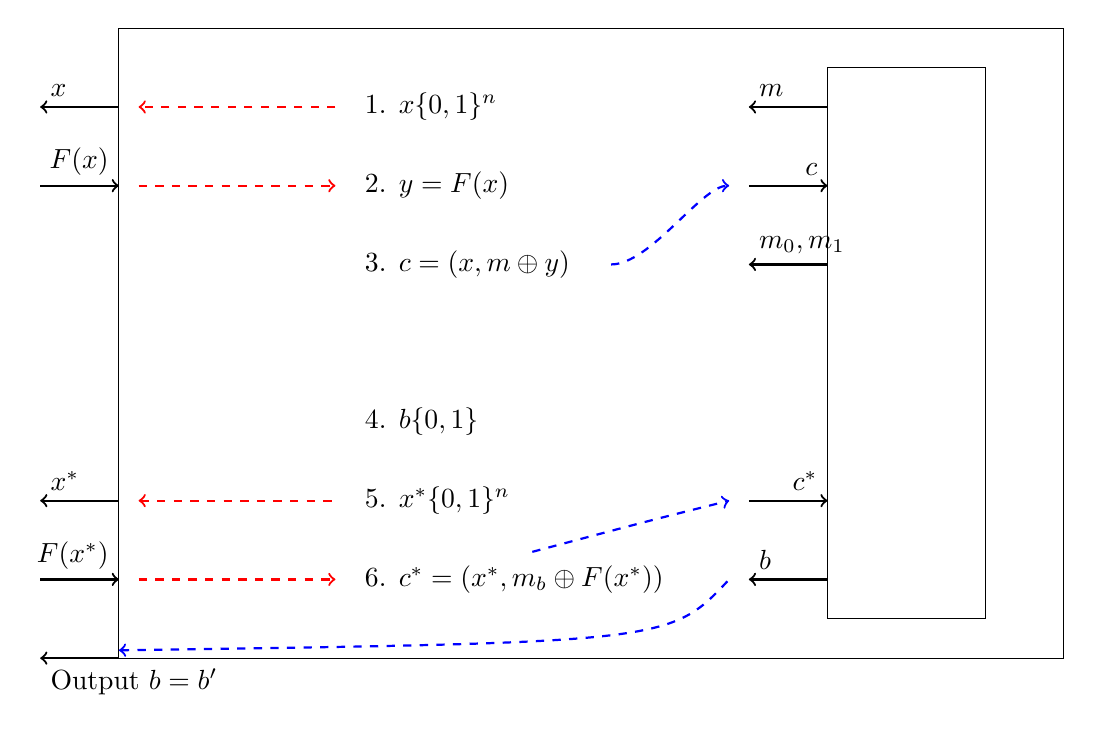
\begin{tikzpicture}
        % Adversary B rectangle
        \draw (0,8) node[anchor=north west]{$\mb$};
        \draw (0, 0) rectangle (12, 8);
        \draw[thick, ->] (0,7)--(-1,7) node[anchor=south west] {$x$};
        \draw[thick, ->] (-1,6)--(0,6) node[anchor=south east] {$F(x)$};
        \draw (9, 0.5) rectangle (11, 7.5);
        % Adversary A rectangle
        \draw (9,7.5) node[anchor=north west]{$\ma$};
        \draw[thick, ->] (0,2)--(-1,2) node[anchor=south west] {$x^*$};
        \draw[thick, ->] (-1,1)--(0,1) node[anchor=south east] {$F(x^*)$};
        \draw[thick, ->] (0,0)--(-1,0) node[anchor=north west] {Output $b = b'$};
        \draw[thick, ->] (9,7)--(8,7) node[anchor=south west] {$m$};
        \draw[thick, ->] (8,6)--(9,6) node[anchor=south east] {$c$};
        \draw[thick, ->] (9,5)--(8,5) node[anchor=south west] {$m_0, m_1$};
        % \draw[thick, ->] (8,4)--(9,4) node[anchor=south east] {$c^*$};
        % \draw[thick, ->] (9,3)--(8,3) node[anchor=south west] {$m$};
        \draw[thick, ->] (8,2)--(9,2) node[anchor=south east] {$c^*$};
        \draw[thick, ->] (9,1)--(8,1) node[anchor=south west] {$b$};
        % Pseudocode
        \draw (3, 7) node[anchor=west] {1. $x \getsr \{0, 1\}^n$};
        \draw (3, 6) node[anchor=west] {2. $y = F(x)$};
        \draw (3, 5) node[anchor=west] {3. $c = (x, m \oplus y)$};
        \draw (3, 3) node[anchor=west] {4. $b \getsr \{0, 1\}$};
        \draw (3, 2) node[anchor=west] {5. $x^* \getsr \{0, 1\}^n$};
        \draw (3, 1) node[anchor=west] {6. $c^* = (x^*, m_b \oplus F(x^*))$};
        % Other arrows
        \draw[thick, dashed, red, ->] (2.75, 7)--(0.25,7);
        
        \draw[thick, dashed, red, ->] (0.25,6)--(2.75, 6);

        \draw[thick, dashed, blue, ->] (6.25, 5) .. controls (6.75, 5) and (7.4, 6) .. (7.75,6);

        \draw[thick, dashed, red, <-] (0.25, 2)--(2.75,2);

        \draw[thick, dashed, red, ->] (0.25, 1)--(2.75,1);

        \draw[thick, dashed, blue, ->] (5.25, 1.35) .. controls (6.75, 1.75) .. (7.75,2);

        \draw[thick, dashed, blue, <-] (0,0.1) .. controls (7, 0.2) .. (7.75, 1);
        
    \end{tikzpicture}
\end{center}
After running this procedure, we guess ``Pseudorandom" if $b=b'$.
Else, we guess random.


Now we argue that 
$$|\Pr[B^{F_n(\cdot)}(1^n) = 1] - \Pr[\mb^{F_n(\cdot)}(1^n) = 1]|$$
is non-negligible.

\begin{align*}
    |\Pr[B^{F_n(\cdot)}(1^n) = 1] - \Pr[\mb^{F_n(\cdot)}(1^n) = 1]| &\ge \frac{1}{2} + \epsilon(n) - (\frac{1}{2} + \frac{q(n)}{2^n}) \\
    &= \epsilon(n) - \frac{q(n)}{2^n}
\end{align*}
\qed

\begin{theorem}
    No deterministic encryption scheme $\Pi$ can be CPA Secure.
\end{theorem}

\proof
The proof of this claim is simple.
If we have a deterministic encryption scheme, then when we get $c^*$, we can again try to encrypt a message and check if $c = c^*$
\qed


\subsection{Counter Mode Encryption}
One construction of a CCA-secure cipher is by the use of the counter mode.

\begin{itemize}
    \item $\enc(k, (m_1,...,m_\ell)):$
    \begin{algorithmic}[1]
        \item $r \getsr \{0,1\}^n$
        \item Output $c = (r, m_1 \oplus F_k(r+1),
            m_2 \oplus F_k(r+2),
            ...,
            m_\ell \oplus F_k(r+\ell))$
    \end{algorithmic}
\end{itemize}

Consider the following picture:

\begin{center}
    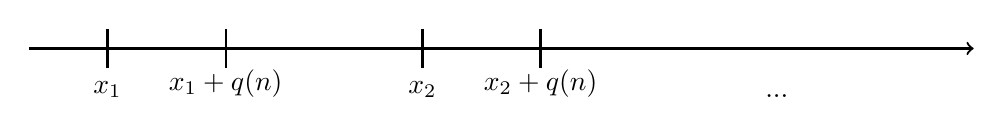
\begin{tikzpicture}
        \draw[thick, ->] (0,0)--(12,0);
        \draw[thick, -] (1, 0.25)--(1, -0.25);
        \draw (1, -0.75) node[anchor=south] {$x_1$};
        \draw[thick, -] (2.5, 0.25)--(2.5, -0.25);
        \draw (2.5, -0.75) node[anchor=south] {$x_1 + q(n)$};
        \draw[thick, -] (5, 0.25)--(5, -0.25);
        \draw (5, -0.75) node[anchor=south] {$x_2$};
        \draw[thick, -] (6.5, 0.25)--(6.5, -0.25);
        \draw (6.5, -0.75) node[anchor=south] {$x_2 + q(n)$};
        \draw (9.5, -0.75) node[anchor=south] {...};
    \end{tikzpicture}
\end{center}

Then the probability of breaking this cipher is
$$\frac{2q(n) - 1}{2^n} \cdot q(n)$$

In practice, we use block ciphers, which are stronger primitives.

\section{Message Authentication Codes}
Now we address the question of how we can guarantee the \textit{integrity} of a message.
To achieve this, we will construct a new primitive, called a \textit{message authentication code}, or MAC for short. MACs generate a verifiable tag $t$ for a message $m$ that cannot be forged.

When sending a message, Alice sends the pair $(m, t)$.
Once Bob receives the message, he runs $\Verify(k, m, t)$.
He accepts the message if $\Verify(k, m, t) = 1$, otherwise he rejects the message.
The formal definition is stated below:
\begin{definition}[Private-Key Encryption Scheme]
    A MAC scheme $\Pi$ is a tuple of algorithms $\Pi = (\gen, \mac, \Verify)$, with the following syntax:
    \begin{enumerate}
        \item $k \leftarrow \gen(1^n)$
        \item $t \leftarrow \mac(k,m)$
        \item $0/1 \leftarrow \Verify(k, m, t)$
    \end{enumerate}
    where $n$ is a security parameter and $k, m \in \{0, 1\}^{l(n)}$
\end{definition}

We impose the following \textit{correctness} requirement on our MACs:
\begin{definition}[MAC Correctness]
    $$\forall n, k \in \gen(1^n), m \in \{0, 1\}^*, \Pr[\Verify(k, m, \mac(k, m)) = 1] = 1$$
\end{definition}

We also want the message authentication codes to be \textit{unforgeable}.
That is, given a message $m$, a nu-PPT attacker $\ma$ should only be able to forge a tag $t$ for $m$ with negligible probability.
\begin{definition}[EUF-CMA Security]
    A MAC scheme $\Pi = (\gen,\mac,\Verify)$ is EUF-CMA-secure if $\forall$ nu-PPT $\ma$,
    $$\Big| \Pr\left[\mathsf{MAC}\pcmathhyphen{}\mathsf{forge}_{\cA, \Pi}(\secpar) =1\right]\Big| = \negl$$
\end{definition}

\begin{definition}[$\mathsf{MAC}\pcmathhyphen{}\mathsf{forge}_{\cA, \Pi}(\secpar)$]
$ $
   \begin{enumerate}
        \item \textbf{Setup:} The challenger samples $k$ uniformly from the key space. $\cA$ is given $1^n$.
        \item \textbf{Query:} The adversary submits a message $m^{(i)}$; then the challenger computes a tag $t^{(i)} \gets \mac(k, m^{(i)})$ and sends it to the adversary. The adversary may submit any polynomial number of message queries.
        
        Let $\mathcal{Q} = \{(m^{(1)}, t^{(1)}), \dots, (m^{(q)}, t^{(q)})\}$ be the set of messages $m^{(i)}$ submitted in the query phase along with the tags $t^{(i)}$ computed by $\mac$.
        \item \textbf{Forgery:} The adversary outputs a message-tag pair $(m^*, t^*)$. The output of the game is $1$ if $(m^*,t^*) \notin \mathcal{Q}$ and $\Verify(k, m^*, t^*) = 1$. The output is $0$ otherwise.
    \end{enumerate}
\end{definition}


%\marginnote[-1.5in]{
%\procedureblock[linenumbering]{$ \pcnotionstyle{OLDPri\pcmathhyphen{}}\indcpa_{\Pi}^{\adv}(\secpar)$}{
% b \sample \bin \\
%  \key  \sample \gen ( \secparam ) \\
% ( \state ,m_0 ,m_1) \sample \adv^{\enc ( \key ,\cdot )} ( \secparam) \\
% c \sample \enc ( \key ,m_b ) \\
% b' \sample \adv^{\enc ( \key ,\cdot )} ( \state , c ) \\
% \pcreturn b = b' }
% }

 
\newcommand{\nonnegl}{\mathsf{nonnegl}}


\section{Fixed-length MACs}

Previously, we defined what a MAC is, and specified correctness and security definitions for MACs. In this section, we'll define a fixed-length MAC for length $\ell(n)$.

\begin{theorem}
    If $F : \{0, 1\}^n \to \{0, 1\}^n$ is a secure PRF, then the MAC scheme $\Pi = (\mathsf{Gen}, \mathsf{Mac}, \mathsf{Verify})$ constructed below has EUF-CMA security.

    \begin{itemize}
        \item $\gen(1^n):$
        \begin{algorithmic}
            \item Output $k \getsr \{0, 1\}^n$
        \end{algorithmic}
        \item $\mac(k,m):$
        \begin{algorithmic}
            \item Output $t = F_k(m)$
        \end{algorithmic}
        \item $\Verify(k, m, t)$
        \begin{algorithmic}
            \item If $t = F_k(m)$, then return $1$. 
            \item Otherwise return $0$.
        \end{algorithmic}
    \end{itemize}
    That is, we just compute the PRF on our message as the MAC.
\end{theorem}

\begin{proof}
    To prove security, suppose for contradiction that there exists an adversary $A$ that breaks the security for $\Pi$. We'd like to construct an adversary $B$ that breaks the security of the PRF.

    Here, the adversary $A$ expects queries for tags, given messages as input. $B$ can simply forward these requests on to $F$, and return the response back to $A$. Further, $A$ outputs a pair $(m^*, t^*)$, which $B$ can send $m^*$ to $F$, and output whether $t = t^*$.

    \begin{center}
        \begin{tikzpicture}
            \draw (3, 0) rectangle (8, 5.5);
            \draw (5, 0.5) rectangle (7.5, 5);
            \node at (3.25, 5.25) {$B$};
            \node at (5.25, 4.75) {$A$};

            \draw (5.5, 4) edge[->] node[right, pos=0] {$m$} (2.5, 4)
                (2.5, 3.5) edge[->] node[right, pos=1] {$t$} (5.5, 3.5);
            \node[left] at (2.5, 3.75) {$F_k$};
            \node at (5.5, 3.1) {$\vdots$};
            \node at (4.5, 3.1) {$\vdots$};
            \draw (5.5, 2.5) edge[->] node[right, pos=0] {$(m^*, t^*)$} (4.5, 2.5);

            \draw (3.5, 2.5) edge[->] node[right, pos=0] {$m^*$} (2.5, 2.5);
            \node[left] at (2.5, 2.25) {$F_k$};
            \draw (2.5, 2) edge[->] node[right, pos=1] {$t$} (3.5, 2);
            \draw (3.5, 1) edge[->] node[right, pos=0] {$t \overset{?}{=} t^*$} (2.5, 1);
        \end{tikzpicture}
    \end{center}

    Analyzing the probability for $B$, we have
    \[
        \abs{\Pr(B^{F_k(\cdot)}(1^n) = 1) - \Pr(B^{R_n(\cdot)}(1^n) = 1)}
        = \abs{\varepsilon_A(n) - \frac{1}{2^n}}
        = \nonnegl(n)
    .\]
    Here, the first term is because the correctness follows immediately from the correctness of $A$, and the second term is due to the fact that the output of $R_n$ is random.
\end{proof}

\section{Variable-length MACs}

Now, let us look at messages with lengths that are a multiple of $n$. In particular, we have a few blocks $m_1, \ldots, m_{\ell}$, each of size $n$. There are a few ways to do this, but we'll look at a method similar to the counter mode we looked at last time.

\begin{center}
    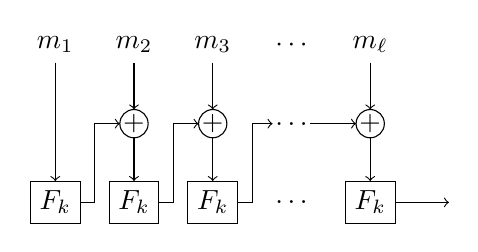
\begin{tikzpicture}
        \node (m1) at (0, 2) {$m_1$};
        \node (m2) at (1, 2) {$m_2$};
        \node (m3) at (2, 2) {$m_3$};
        \node (mdots) at (3, 2) {$\cdots$};
        \node (ml) at (4, 2) {$m_{\ell}$};

        \node[draw] (fk1) at (0, 0) {$F_k$};
        \node[draw] (fk2) at (1, 0) {$F_k$};
        \node[draw] (fk3) at (2, 0) {$F_k$};
        \node at (3, 0) {$\ldots$};
        \node[draw] (fkl) at (4, 0) {$F_k$};

        \node[outer sep=0pt, inner sep=0pt, draw, circle] (fk1+m2) at (1, 1) {$+$};
        \node[outer sep=0pt, inner sep=0pt, draw, circle] (fk2+m3) at (2, 1) {$+$};
        \node[outer sep=0pt, inner sep=1pt] (xor-dots) at (3, 1) {$\ldots$};
        \node[outer sep=0pt, inner sep=0pt, draw, circle] (dots+ml) at (4, 1) {$+$};

        \draw (m1) edge[->] (fk1)
            (m2) edge[->] (fk1+m2)
            (m3) edge[->] (fk2+m3)
            (ml) edge[->] (dots+ml);

        \draw[->] (fk1) -- ++(0.5, 0) |- (fk1+m2);
        \draw[->] (fk2) -- ++(0.5, 0) |- (fk2+m3);
        \draw[->] (fk3) -- ++(0.5, 0) |- (xor-dots);

        \draw[->] (xor-dots) -- (dots+ml);
        \draw (fk1+m2) edge[->] (fk2)
            (fk2+m3) edge[->] (fk3)
            (dots+ml) edge[->] (fkl);
        \draw (fkl) edge[->] ++(1, 0);
    \end{tikzpicture}
\end{center}

This construction avoids having to store a tag equal in length to the message, but this is not secure, due to length extension attacks. In particular, suppose we query for the tag $t$ associated with $0^n$. We can then query another tag $t'$ for $0^n \oplus t$. Observe here that $t'$ is also the tag for $0^{2n}$.

A solution is to use different keys for each PRF, but this isn't too efficient, since we're still calling the PRF once per block of length $n$. We'll instead improve this to use only one block cipher call---we do some preprocessing and only call $F_k$ once on the output of the preprocessing.

In particular, we'll claim that applying a universal hash function to the input and then applying the block cipher is a secure MAC.

\begin{definition}[Universal Hash Function]
    A function $h : \mathcal{F} \times \mathcal{F}^* \to \mathcal{F}$ (where $\mathcal{F}$ is a field of size $2^m$) is a universal hash function if for all $m, m' \in \mathcal{F}^{\le \ell}$ (i.e. $m$ and $m'$ have length at most $\ell$),
    \[
        \Pr_s(h(s, m) = h(s, m')) \le \frac{\ell}{\abs{F}}
    .\]
    That is, the probability of collision is small.
\end{definition}

Crucially here, we fix $m$ and $m'$, and we sample $s$. (If we fix an $s$, we can almost surely find an $m$ and $m'$ that collide.)

Today, we'll look at the following function:
\[
    h(s, m_0, \ldots, m_{\ell - 1}) = m_0 + m_1 s + m_2 s^2 + \cdots + m_{\ell - 1} s^{\ell - 1} + s^{\ell}
.\]

\begin{claim}
    The function defined by
    \[
        h(s, m_0, \ldots, m_{\ell - 1}) = m_0 + m_1 s + m_2 s^2 + \cdots + m_{\ell - 1} s^{\ell - 1} + s^{\ell}
    \]
    is a universal hash function.
\end{claim}

\begin{proof}
    We'd like to argue that for a fixed $m$ and $m'$, and a random $s$, the probability that there is a collision is at most $\frac{\ell}{\abs{\mathcal{F}}}$.

    We'll look at
    \[
        h(x, m_0, \ldots, m_t) - h(x, m_0', \ldots, m_t') = (m_0 - m_0') + \cdots + (m_{t - 1} - m_{t-1}') x^{\ell - 1}
    .\]
    If there is a collision, this difference is 0. The probability that this polynomial of degree at most $\ell$ has a zero at $x$ is at most $\frac{\ell}{\abs{\mathcal{F}}}$, since it has at most $\ell$ zeroes. This means that $h$ is indeed a universal hash function.
\end{proof}

\begin{claim}
    The MAC given by $F_k(h(s, m_1, \ldots, m_{\ell}))$, for the universal hash function $h$ given prior, is secure. (This is a slight variation on the Carter--Wegman MAC.)
\end{claim}

\begin{proof}
    Suppose for contradiction that there exists a nu-PPT $A$ that breaks the security of this scheme.

    Here, for appropriately generated $k$ and $s$, $A$ makes queries $m \mapsto F_k(h_s(m))$, and outputs $(m^*, t^*)$.

    We'd like to create an adversary $B$ that either breaks the security of the PRF, or breaks the security of the universal hash function.

    $B$ will start by sampling $s \in \mathcal{F}$. When given the query for $m_1$, it computes $h_s(m_1)$ and queries for $F_k(h_s(m_1))$, which it sends back to $A$. If $F_k$ was actually pseudorandom, then $A$ is given a pseudorandom input, and if $F_k$ was random $R_n$, then $A$ is given a random input.

    $A$ must still be able to generate pairs $(m^*, t^*)$ even when given a random input, due to the security of the PRF.

    \begin{center}
        \begin{tikzpicture}
            \draw (2, 0) rectangle (8, 5.5);
            \draw (5, 0.5) rectangle (7.5, 5);
            \node at (2.25, 5.25) {$B$};
            \node at (5.25, 4.75) {$A$};

            \node at (3.5, 4.5) {sample $s \in \mathcal{F}$};

            \node (hsm) at (3.5, 4) {$h_s(m)$};
            \draw (5.5, 4) edge[->] node[right, pos=0] {$m$} (hsm)
                (hsm) edge[->] (1.5, 4)
                (1.5, 3.5) edge[->] node[right, pos=1] {$t$} (5.5, 3.5);
            \node[left] at (1.5, 3.75) {$F_k$};
            \node at (5.5, 3.1) {$\vdots$};
            \node at (4.5, 3.1) {$\vdots$};

            \node (hash-m-star) at (3.5, 2.5) {$h_s(m^*)$};
            \draw (5.5, 2.5) edge[->] node[right, pos=0] {$(m^*, t^*)$} (hash-m-star)
                (hash-m-star) edge[->] (1.5, 2.5);
            \node[left] at (1.5, 2.25) {$F_k$};
            \draw (1.5, 2) edge[->] node[right, pos=1] {$t$} (3.5, 2);
            \draw (3.5, 1) edge[->] node[right, pos=0] {$t \overset{?}{=} t^*$} (1.5, 1);
        \end{tikzpicture}
    \end{center}

    Let $E$ be the event that there exists an $m, m' \in L \cup \{m^*\}$, such that $h_s(m) = h(m')$. If $E$ does not happen, then the hash function never collides. This means that the attacker only sees random values depending on distinct inputs, so this reduces to the case from earlier (when the MAC is just $F_k$).

    As such, we'd like to show that collisions in $h_s(\cdot)$ occur with negligible probability.

    To show this, suppose for contradiction that collisions actually do occur with non-negligible probability. We then want to construct an adversary $B$ utilizing $A$ that just outputs $m$ and $m'$ such that when $s$ is sampled, $h_s(m) = h_s(m')$ with high probability.

    $B$ will pick a random $i, j \in \{1, \ldots, q+1\}$ (here suppose $i < j$), where $q$ is the number of MAC queries. We then run $A$ until the $j$th query. Taking the $i$th and $j$th query, we then output $m_i$ and $m_j$ as our pair of messages. We still need to entertain the queries made by $A$, so we can just return random values for tags (giving the same value if it requests it for the same message).

    \begin{center}
        \begin{tikzpicture}
            \draw (2, 0) rectangle (8, 6);
            \draw (5, 0.5) rectangle (7.5, 5.5);
            \node at (2.25, 5.75) {$B$};
            \node at (5.25, 5.25) {$A$};

            \node[align=center] at (3.5, 5) {\small $i, j \xleftarrow{\$} \{1, \ldots, q+1\}$};

            \draw (5.5, 4) edge[->] node[right, pos=0] {$m_1$} (4.5, 4)
                (4.5, 3.5) edge[->] node[left, pos=0] {sample $t_1$} node[right, pos=1] {$t_1$} (5.5, 3.5);
            \node at (5.5, 3.1) {$\vdots$};
            \node at (4.5, 3.1) {$\vdots$};

            \draw (5.5, 2.5) edge[->] node[right, pos=0] {$m_i$} (4.5, 2.5)
                (4.5, 2) edge[->] node[left, pos=0] {sample $t_i$} node[right, pos=1] {$t_i$} (5.5, 2);
            \node at (5.5, 1.6) {$\vdots$};
            \node at (4.5, 1.6) {$\vdots$};

            \draw (5.5, 1) edge[->] node[right, pos=0] {$m_j$} (4.5, 1);

            \draw (3, 0.5) edge[->] node[right, pos=0] {$(m_i, m_j)$} (1.5, 0.5);
        \end{tikzpicture}
    \end{center}

    By assumption, we know that $E$ occurs with non-negligible probability. That is, among the queries made by $A$, there is a non-negligible probability that $h_s(m_i) = h_s(m_j)$. Since here the implementation of $B$ just picks out a pair of random queries from those made by $A$, the pair $(m_i, m_j)$ output by $B$ also has a collision with non-negligible probability. (In particular, with probability $\Pr(E) / q^2$.

    This breaks the definition of a universal hash function, which is a contradiction.
\end{proof}

So far, we know how to generate tags of fixed length, and of lengths that are a multiple of $n$. If we have a message that is not a multiple of $n$, we could potentially just pad the input with 0's, but this causes an issue, as $m$ and $m \concat 0$ have the same tag.

Instead, one solution is to put the size of the message in the first block, and we can still put the padding at the end. This way, if the messages differ by length, the first block will be different, and if the messages do not differ by length, then we're essentially just ignoring the padding. This gives us a MAC for arbitrary-length messages.

\section{Authenticated Encryption Schemes}

We've talked about confidentiality and integrity separately, but generally we want both properties---when Alice sends a message to Bob, we'd like for any eavesdropper to be unable to recover the message, \emph{and} we'd like Bob to be able to verify that the message actually came from Alice.

A scheme that achieves both of these conditions is called an \emph{authenticated encryption scheme}.

\begin{definition}[Authenticated Encryption Scheme]
    A scheme $\Pi$ is an \emph{authenticated encryption scheme} if it is CPA-secure, and it has ciphertext integrity (CI).
\end{definition}

\begin{definition}[Ciphertext Integrity (CI)]
    Consider the following game for the scheme $\Pi = (\mathsf{Gen}, \mathsf{Enc}, \mathsf{Dec})$.

    \begin{algorithmic}[1]
        \Function{CI${}_{\Pi}^A$}{$n$}
            \State $k \gets \mathsf{Gen}(1^n)$
            \State $c^* \gets A^{\mathsf{Enc}(k, \cdot)}(1^n)$
            \State $L \gets$ the list of queries made by $A$
            \State \Return $(\mathsf{Dec}(k, c^*) \ne \bot) \land (c^* \notin L)$
        \EndFunction
    \end{algorithmic}

    A scheme has ciphertext integrity if for all nu-PPT $A$, $\Pr(\mathrm{CI}_{\Pi}^A)$ is negligible.
\end{definition}

Observe that an authenticated encryption scheme is also CCA-secure, since the CI property says that the adversary can never generate a valid ciphertext. This means that whenever an adversary requests the decryption of a ciphertext, we can always return $\bot$ (unless they previously requested a ciphertext for a message, and wants to decode that ciphertext). This means that the decryption oracle is essentially useless, and this reduces to the CPA case.

Next, we'll construct an authenticated encryption scheme, called ``Encrypt-then-MAC'', utilizing a CPA-secure encryption scheme and an EUF-CMA MAC scheme.

\begin{claim}
    Let $\Pi_e = (\mathsf{Gen}_e, \mathsf{Enc}_e, \mathsf{Dec}_e)$ be a CPA-secure encryption scheme, and let $\Pi_m = (\mathsf{Gen}_m, \mathsf{Mac}_m, \mathsf{Verify}_m)$ be an EUF-CMA-secure MAC scheme.

    The following scheme $\Pi = (\mathsf{Gen}, \mathsf{Enc}, \mathsf{Dec})$ is an authenticated encryption scheme.

    \begin{algorithmic}[1]
        \Function{Gen}{$1^n$}
            \State $k_e \gets \mathsf{Gen}_e(1^n)$
            \State $k_m \gets \mathsf{Gen}_m(1^n)$
            \State \Return $(k_e, k_m)$
        \EndFunction
        \Statex
        \Function{Enc}{$(k_e, k_m), m$}
            \State $c \gets \mathsf{Enc}_e(k_e, m)$
            \State $t \gets \mathsf{Mac}_m(k_m, c)$
            \State \Return $(c, t)$
        \EndFunction
        \Statex
        \Function{Dec}{$(k_e, k_m), (c, t), m$}
            \If {$\mathsf{Verify}_m(k_m, c, t)$}
                \State \Return $\mathsf{Dec}_e(k_e, c)$
            \Else
                \State \Return $\bot$
            \EndIf 
        \EndFunction
    \end{algorithmic}
\end{claim}

\begin{proof}
    Suppose for contradiction that we have an adversary $A$ that breaks the CPA security of $\Pi$. The CPA game allows for queries of the ciphertext for messages $m$, produces a pair $m_0, m_1$, and then gets $c^* = \mathsf{Enc}(k, m_B)$, and $A$ eventually outputs $b'$ to identify which message was encrypted.

    We'd like to construct another adversary $B$, which breaks the CPA-security of $\Pi_e$. The only difference here is the MACs, so $B$ can sample a $k_m \gets \mathsf{Gen}_m(1^n)$, and perform all of the MACs itself.

    In particular, when $A$ asks for the ciphertext of $M$, we pass it to the oracle for $\Pi_e$, and attach $t \gets \mathsf{Mac}_m(k_m, c)$. If $A$ is able to distinguish between ciphertexts of $M_0$ and $M_1$, then we can use the same bit to distinguish between ciphertexts for $\Pi_e$.
    \begin{center}
        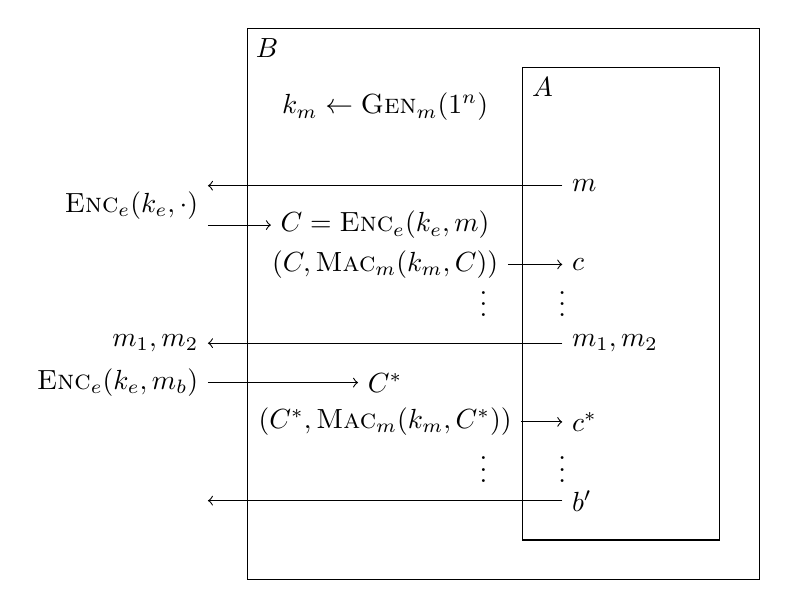
\begin{tikzpicture}
            \draw (1.5, -1) rectangle (8, 6);
            \draw (5, -0.5) rectangle (7.5, 5.5);
            \node at (1.75, 5.75) {$B$};
            \node at (5.25, 5.25) {$A$};

            \node at (3.25, 5) {$k_m \gets \textsc{Gen}_m(1^n)$};

            \node (enc) at (3.25, 3.5) {$C = \textsc{Enc}_e(k_e, m)$};
            \node (mac) at (3.25, 3) {$(C, \textsc{Mac}_m(k_m, C))$};

            \draw (5.5, 4) edge[->] node[right, pos=0] {$m$} (1, 4)
                (1, 3.5) edge[->] (enc)
                (mac) edge[->] node[right, pos=1] {$c$} (5.5, 3);
            \node[left] at (1, 3.75) {$\textsc{Enc}_e(k_e, \cdot)$};
            \node at (5.5, 2.6) {$\vdots$};
            \node at (4.5, 2.6) {$\vdots$};

            \draw (5.5, 2) edge[->] node[right, pos=0] {$m_1, m_2$} node[left, pos=1] {$m_1, m_2$} (1, 2);
            \node (enc-mb) at (3.25, 1.5) {$C^*$};
            \node (mac-mb) at (3.25, 1) {$(C^*, \textsc{Mac}_m(k_m, C^*))$};
            \draw (1, 1.5) edge[->] node[left, pos=0] {$\textsc{Enc}_e(k_e, m_b)$} (enc-mb);
            \draw (mac-mb) edge[->] node[right, pos=1] {$c^*$} (5.5, 1);

            \node at (5.5, 0.5) {$\vdots$};
            \node at (4.5, 0.5) {$\vdots$};

            \draw (5.5, 0) edge[->] node[right, pos=0] {$b'$} (1, 0);
        \end{tikzpicture}
    \end{center}

    To prove ciphertext integrity, suppose we have an adversary $A$ that breaks the ciphertext integrity of $\Pi$. Here, $A$ asks for ciphertext queries, and eventually returns a new ciphertext that is valid.

    We'd like to construct an adversary $B$ that is able to generate a new message and a tag, given oracle access to the MAC scheme. The construction will follow similarly to the prior proof on CPA security.

    Here, our adversary $B$ can sample $k_e \gets \mathsf{Gen}_e(1^n)$. When $A$ asks for the encryption of $M$, $B$ can send $m = \mathsf{Enc}_e(k_e, M)$ to the MAC oracle, and it returns $c = (m, t)$ to $A$.

    When $A$ returns $C^* = (c^*, t^*)$, $B$ can also just return the same, since the tag $t^*$ is being computed on $c^*$.

    \begin{center}
        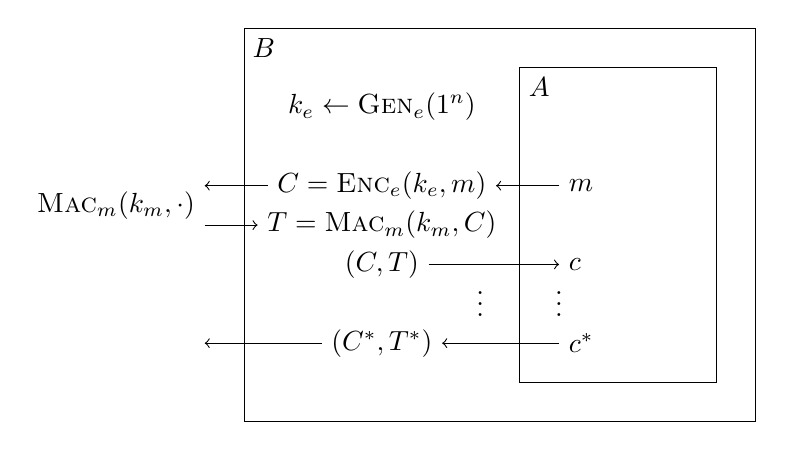
\begin{tikzpicture}
            \draw (1.5, 1) rectangle (8, 6);
            \draw (5, 1.5) rectangle (7.5, 5.5);
            \node at (1.75, 5.75) {$B$};
            \node at (5.25, 5.25) {$A$};

            \node at (3.25, 5) {$k_e \gets \textsc{Gen}_e(1^n)$};

            \node (enc) at (3.25, 4) {$C = \textsc{Enc}_e(k_e, m)$};
            \node (mac) at (3.25, 3.5) {$T = \textsc{Mac}_m(k_m, C)$};
            \node (enc-mac) at (3.25, 3) {$(C, T)$};

            \draw (5.5, 4) edge[->] node[right, pos=0] {$m$} (enc)
                (enc) edge[->] (1, 4)
                (1, 3.5) edge[->] (mac)
                (enc-mac) edge[->] node[right, pos=1] {$c$} (5.5, 3);
            \node[left] at (1, 3.75) {$\textsc{Mac}_m(k_m, \cdot)$};
            \node at (5.5, 2.6) {$\vdots$};
            \node at (4.5, 2.6) {$\vdots$};

            \node (gen-ciphertext) at (3.25, 2) {$(C^*, T^*)$};
            \draw (5.5, 2) edge[->] node[right, pos=0] {$c^*$} (gen-ciphertext)
                (gen-ciphertext) edge[->] (1, 2);
        \end{tikzpicture}
    \end{center}
\end{proof}

As an example, AES-GCM is the most popular authenticated encryption scheme that is used, and also has the ability to authenticate additional data. (AES-GCM basically just appends the associated data to the ciphertext, so that the encryption is only on the message, but the MAC is on both the ciphertext and the associated data.) This scheme uses a counter-mode encryption scheme, and the MAC that we saw, but makes this more efficient.



